\chapter{Hipótesis}

La hipótesis que se maneja en este estudio se basa en la suposici\'on de que la materia oscura está compuesta de partículas elementales las cuales pueden ser producidas
en los laboratorios modernos de fisica de particulas.
De ser esto cierto se requiere de un nuevo marco teórico, es decir una extension al modelo estandar que sustente dicha hipótesis. Afortunadamente ya se cuenta con modelos bien fundamentas que predicen dicha producción, uno de los modelos más populares es el conocido como "dark SUSY"~\cite{} en el cual existe un llamado sector oscuro donde por
medio del rompimiento del grupo de simetria $U(1)_{D}$ se da lugar a la creacion de fotones oscuros ($\gamma_{D}$) ligeros, los cuales interactuarían con partículas
del modelo estandar y dicha fuerza de interaccion estaria descrita por medio de un parametro de mezcla cinetico $\epsilon$.  Una representacion grafica entre el sector oscuro y el del modelo estandar representa
en la la Figura~\ref{fig:sketch_darksector} (izquierda). En "dark SUSY" ademas de particulas de materia oscura se da lugar a la producccion de particulas supersimetricas (SUSY), en donde la mas ligera de estas, el neutralino, dejaria de ser estable y podria decaer al foton oscuro. Las nuevas fuerzas en "dark SUSY" estarian mediadas mediante
un termino de acoplamiento a la hypercarga del modelo estandar, descrito por la siguiente ecuacion.  

\begin{equation} 
L_{KM} = \frac{\epsilon}{2} F_{\mu\nu}^{\gamma}F^{D_{\mu\nu}}
\end{equation}

Donde $F_{\mu\nu}^{D}$ representa el campo oscuro.  Debido a la interaccion descrita por $\epsilon$ el foton oscuro puede decaer a leptones del Modelo Standar
con una amplitud de decaimiento dada por:

\begin{equation}
  \Gamma_{\gamma D \rightarrow ll} = \frac{1}{3}\alpha \epsilon^{2} m_{\gamma D} \sqrt{1-\frac{4 m_{l}^{2}}{m_{\gamma D}^2}}(1+\frac{2m_{l}^{2}}{m_{\gamma D}}^{2})
\end{equation}

La expresion para las amplitudes permite calcular el tiempo de vida del fotos oscuro dado por: 

\begin{equation}
  \tau_{\gamma D}= \frac{\hbar}{\Gamma_{\gamma D Total}}=\frac{1}{\Gamma_{\gamma D \rightarrow e^{+}e^{-}}  + \Gamma_{\gamma D \rightarrow \mu^{+}\mu^{-}} + \Gamma_{\gamma D \rightarrow hadrons}}
\end{equation}

%%% EScribir la ecuacion. 

\begin{figure}
    \centering
    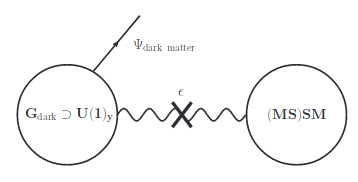
\includegraphics[width=0.4\textwidth]{HIPOTESIS/sketch_darksector.png}
    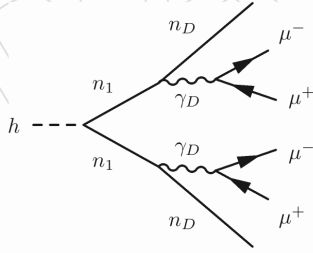
\includegraphics[width=0.4\textwidth]{HIPOTESIS/darksusy_feynman.png}
    \caption{. Ilustración esquemática de la conexión entre el sector oscuro y el modelo estándar, los cuales están conectados mediante un término de mezcla dinámica.}
    \label{fig:sketch_darksector}
\end{figure}


El diagrama de Feynman para el proceso del modelo "dark SUSY" $h\rightarrow 2n_{1}\rightarrow 2n_{D}\rightarrow 2\gamma_{D} \rightarrow 2n_{D} + 4\mu$ se muestra en la figura~\ref{fig:sketch_darksector} (derecha). 

Este escenario simple "dark SUSY" podria ser extendido de diversas maneras, por ejemplo, versiones mas complejas podrian involucrar otras particulas del sector oscuro como Higgs oscuros, o bosones Z y W oscuros, dando cabida a procesos como $pp\rightarrow h \rightarrow Z_{D}Z/Z_{D}Z_{D}/Z_{a}\rightarrow 4\mu$. Sin embargo dichos modelos escapan a los alcances de esta tesis y podrian ser explorados en un analsis futuro. 















